\documentclass[11pt]{article}
\usepackage[margin=1in]{geometry}
\usepackage{graphicx}
\usepackage{float}
\usepackage{booktabs}
\usepackage{siunitx}
\usepackage{amsmath}
\usepackage{amssymb}
\usepackage{pgfplots}
\usepackage{listings}
\usepackage{xcolor}

\pgfplotsset{compat=1.18}

% Code listing style configuration
\definecolor{codegreen}{rgb}{0,0.6,0}
\definecolor{codegray}{rgb}{0.5,0.5,0.5}
\definecolor{codepurple}{rgb}{0.58,0,0.82}
\definecolor{backcolour}{rgb}{0.95,0.95,0.92}

\lstdefinestyle{mystyle}{
  backgroundcolor=\color{backcolour},
  commentstyle=\color{codegreen},
  keywordstyle=\color{magenta},
  numberstyle=\tiny\color{codegray},
  stringstyle=\color{codepurple},
  basicstyle=\ttfamily\footnotesize,
  breakatwhitespace=false,
  breaklines=true,
  captionpos=b,
  keepspaces=true,
  numbers=left,
  numbersep=5pt,
  showspaces=false,
  showstringspaces=false,
  showtabs=false,
  tabsize=2
}
\lstset{style=mystyle}

\title{\textbf{ENGR 200: Lab 4}\\
Signal Analysis and Data Acquisition}
\author{Sean Balbale}
\date{March 2026}
\setlength{\parindent}{0in}
\setlength{\parskip}{\baselineskip}

\begin{document}

\begin{titlepage}
  \begin{center}
    \vspace*{1in}

    \Huge
    \textbf{Lab 4}

    \LARGE
    Signal Analysis and Data Acquisition

    \vspace{3in}

    \textbf{Student Name:} Sean Balbale
    \\ \textbf{Course:} Engineering 200
    \\ \textbf{Instructor:} Prof. R. Gao
    \\ \textbf{Date:} March 13, 2026

    \vfill

  \end{center}
\end{titlepage}

\newpage

\section*{Part 1: Data Presentation}

The following section pairs the time-domain waveform with its corresponding frequency-domain power spectrum for all eight tested signals. The power spectrums are plotted utilizing a \textbf{logarithmic y-axis (dB)} to properly visualize the dynamic range between the fundamental frequency power and the lower-energy harmonics.

% ---------------------------------------------------------
% Signal 1: Sine 7Hz
% ---------------------------------------------------------
\subsection*{1. Sine Wave: \SI{7}{\hertz}, \SI{5.0}{V_{pp}}, \SI{0.0}{V} Offset}

\begin{figure}[H]
  \centering
  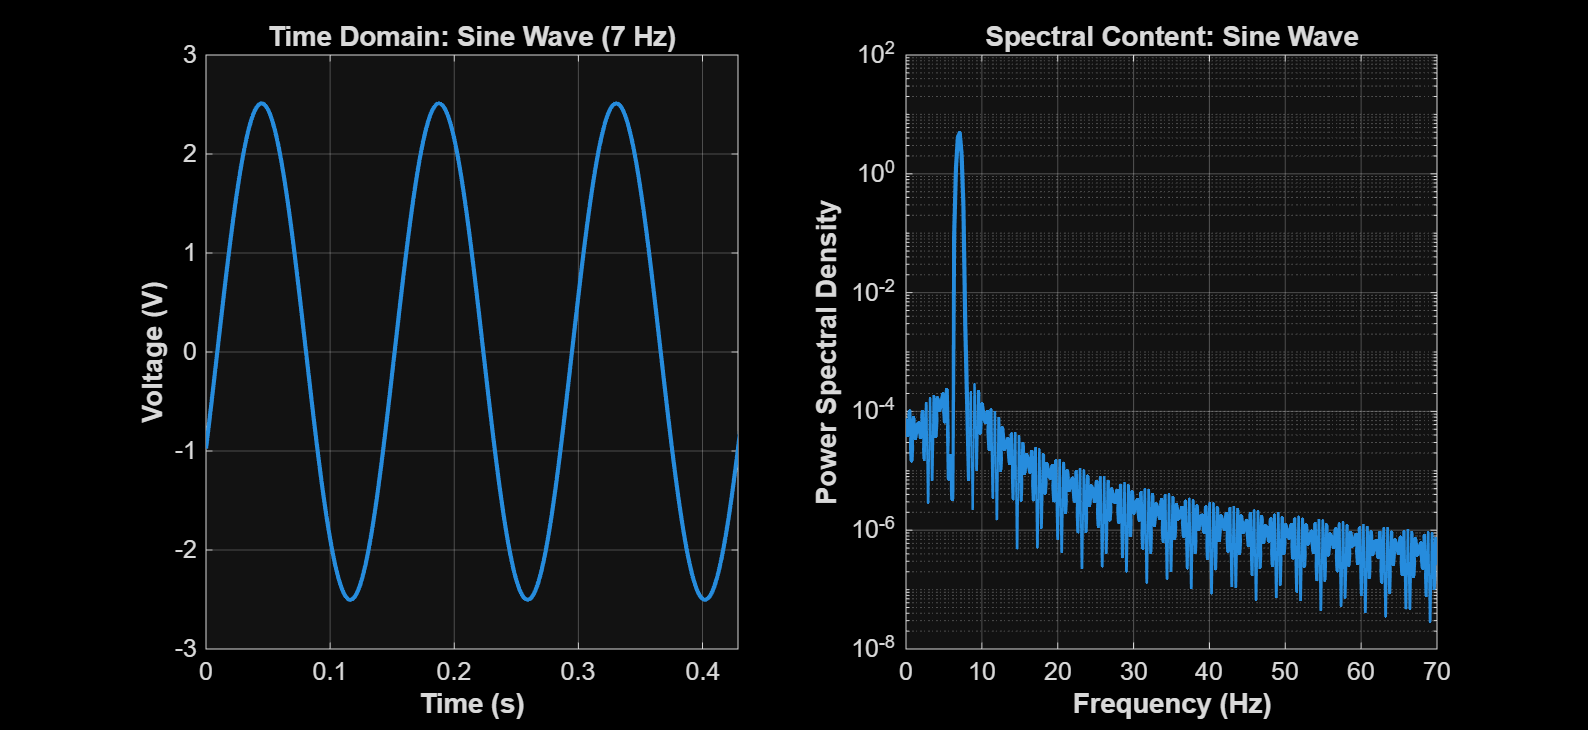
\includegraphics[width=0.9\textwidth]{../pictures/Sine_7Hz_5.0Vpp_0.0Voffset.png}
  \caption{Sine Wave (\SI{7}{\hertz}) Analysis. Time-domain waveform (left) and logarithmic power spectrum (right).}
\end{figure}

\begin{table}[H]
  \centering
  \begin{tabular}{ccc}
    \toprule
    \textbf{Mean Voltage} & \textbf{RMS Voltage} & \textbf{DC Offset} \\
    \midrule
    \SI{0.0042}{\volt} & \SI{1.7722}{\volt} & \SI{0.0042}{\volt} \\
    \bottomrule
  \end{tabular}
\end{table}

% ---------------------------------------------------------
% Signal 2: Sine 25Hz
% ---------------------------------------------------------
\subsection*{2. Sine Wave: \SI{25}{\hertz}, \SI{0.3}{V_{pp}}, \SI{0.2}{V} Offset}

\begin{figure}[H]
  \centering
  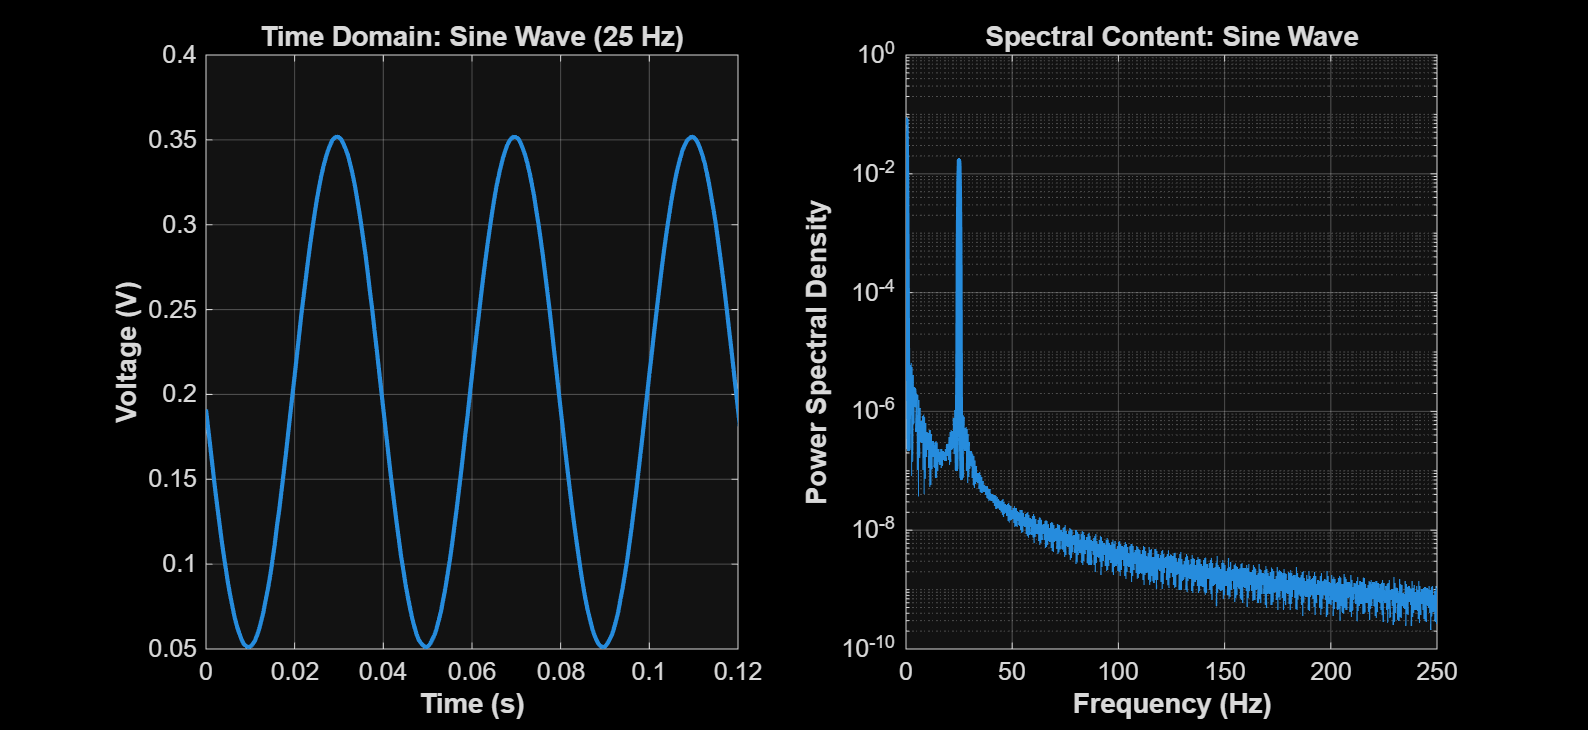
\includegraphics[width=0.9\textwidth]{../pictures/Sine_25Hz_0.3Vpp_0.2Voffset.png}
  \caption{Sine Wave (\SI{25}{\hertz}) Analysis. Time-domain waveform (left) and logarithmic power spectrum (right).}
\end{figure}

\begin{table}[H]
  \centering
  \begin{tabular}{ccc}
    \toprule
    \textbf{Mean Voltage} & \textbf{RMS Voltage} & \textbf{DC Offset} \\
    \midrule
    \SI{0.2014}{\volt} & \SI{0.2277}{\volt} & \SI{0.2014}{\volt} \\
    \bottomrule
  \end{tabular}
\end{table}

% ---------------------------------------------------------
% Signal 3: Triangle (50% Ramp) 7Hz
% ---------------------------------------------------------
\subsection*{3. Ramp Wave (50\% Symmetry): \SI{7}{\hertz}, \SI{5.0}{V_{pp}}, \SI{0.0}{V} Offset}

\begin{figure}[H]
  \centering
  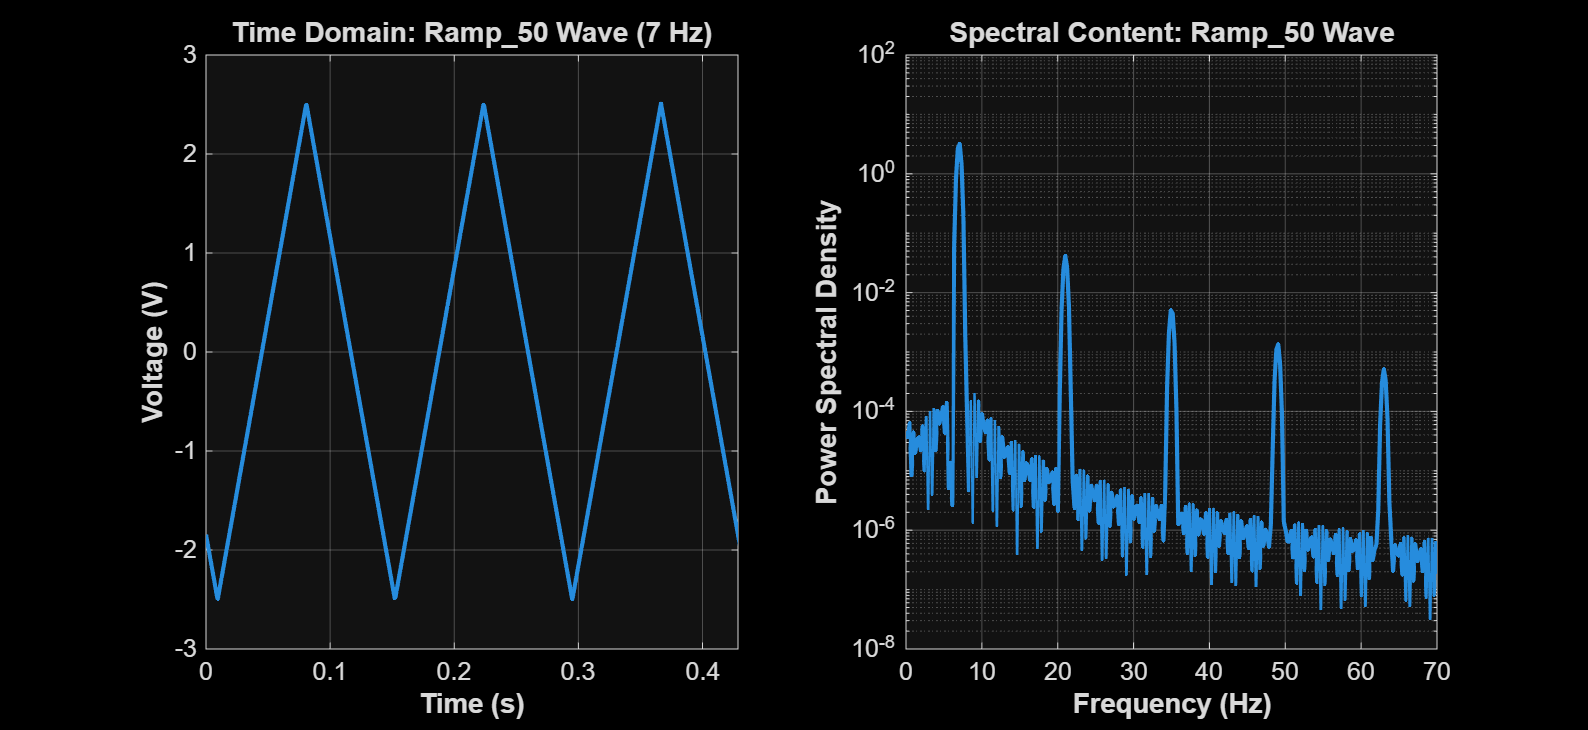
\includegraphics[width=0.9\textwidth]{../pictures/Ramp_50_7Hz_5.0Vpp_0.0Voffset.png}
  \caption{50\% Ramp/Triangle Wave (\SI{7}{\hertz}) Analysis.}
\end{figure}

\begin{table}[H]
  \centering
  \begin{tabular}{ccc}
    \toprule
    \textbf{Mean Voltage} & \textbf{RMS Voltage} & \textbf{DC Offset} \\
    \midrule
    \SI{0.0040}{\volt} & \SI{1.4471}{\volt} & \SI{0.0040}{\volt} \\
    \bottomrule
  \end{tabular}
\end{table}

% ---------------------------------------------------------
% Signal 4: Triangle (50% Ramp) 25Hz
% ---------------------------------------------------------
\subsection*{4. Ramp Wave (50\% Symmetry): \SI{25}{\hertz}, \SI{0.3}{V_{pp}}, \SI{0.2}{V} Offset}

\begin{figure}[H]
  \centering
  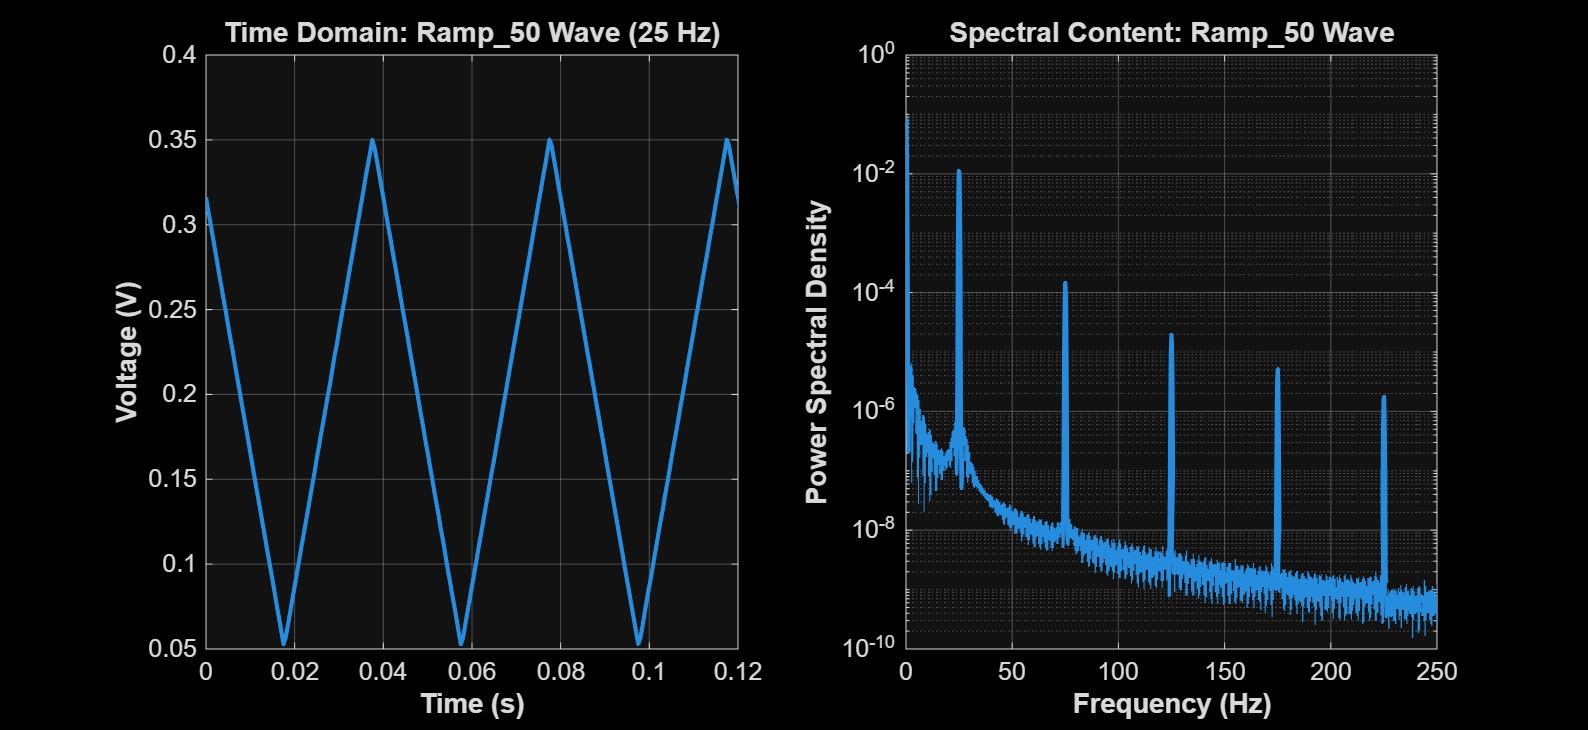
\includegraphics[width=0.9\textwidth]{../pictures/Ramp_50_25Hz_0.3Vpp_0.2Voffset.png}
  \caption{50\% Ramp/Triangle Wave (\SI{25}{\hertz}) Analysis.}
\end{figure}

\begin{table}[H]
  \centering
  \begin{tabular}{ccc}
    \toprule
    \textbf{Mean Voltage} & \textbf{RMS Voltage} & \textbf{DC Offset} \\
    \midrule
    \SI{0.2014}{\volt} & \SI{0.2193}{\volt} & \SI{0.2014}{\volt} \\
    \bottomrule
  \end{tabular}
\end{table}

% ---------------------------------------------------------
% Signal 5: Sawtooth (100% Ramp) 7Hz
% ---------------------------------------------------------
\subsection*{5. Ramp Wave (100\% Symmetry): \SI{7}{\hertz}, \SI{5.0}{V_{pp}}, \SI{0.0}{V} Offset}

\begin{figure}[H]
  \centering
  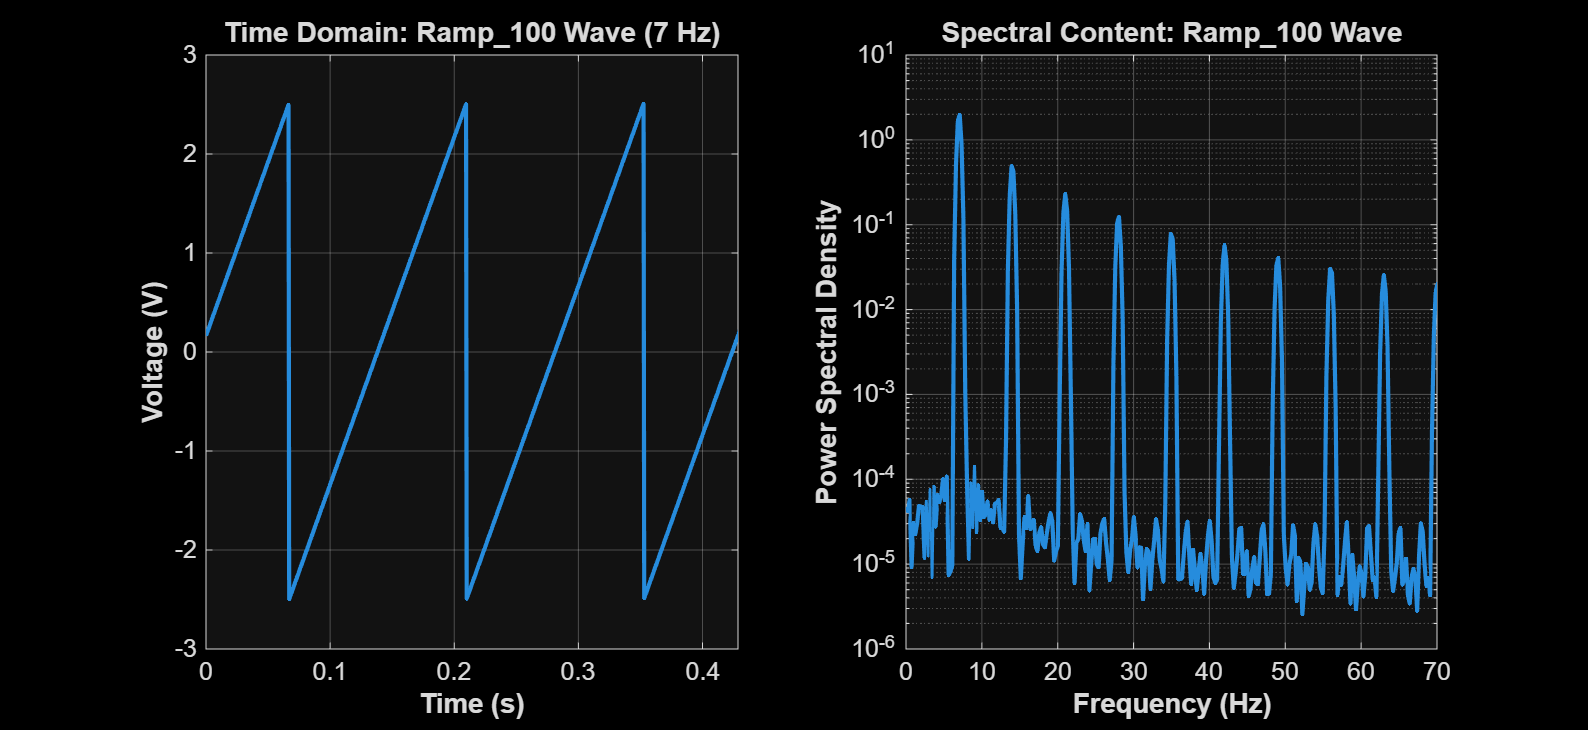
\includegraphics[width=0.9\textwidth]{../pictures/Ramp_100_7Hz_5.0Vpp_0.0Voffset.png}
  \caption{100\% Ramp/Sawtooth Wave (\SI{7}{\hertz}) Analysis.}
\end{figure}

\begin{table}[H]
  \centering
  \begin{tabular}{ccc}
    \toprule
    \textbf{Mean Voltage} & \textbf{RMS Voltage} & \textbf{DC Offset} \\
    \midrule
    \SI{0.0040}{\volt} & \SI{1.4470}{\volt} & \SI{0.0040}{\volt} \\
    \bottomrule
  \end{tabular}
\end{table}

% ---------------------------------------------------------
% Signal 6: Sawtooth (100% Ramp) 25Hz
% ---------------------------------------------------------
\subsection*{6. Ramp Wave (100\% Symmetry): \SI{25}{\hertz}, \SI{0.3}{V_{pp}}, \SI{0.2}{V} Offset}

\begin{figure}[H]
  \centering
  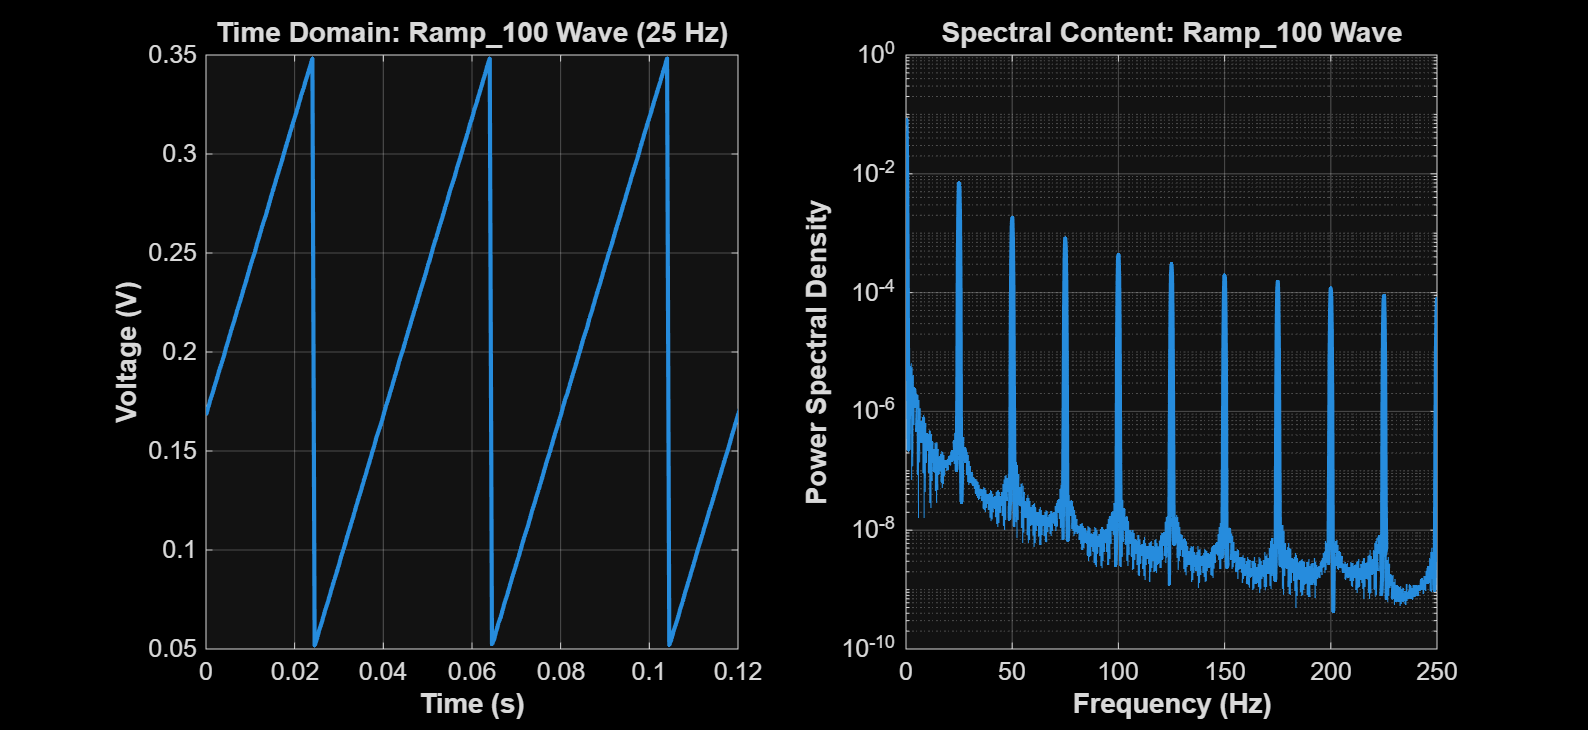
\includegraphics[width=0.9\textwidth]{../pictures/Ramp_100_25Hz_0.3Vpp_0.2Voffset.png}
  \caption{100\% Ramp/Sawtooth Wave (\SI{25}{\hertz}) Analysis.}
\end{figure}

\begin{table}[H]
  \centering
  \begin{tabular}{ccc}
    \toprule
    \textbf{Mean Voltage} & \textbf{RMS Voltage} & \textbf{DC Offset} \\
    \midrule
    \SI{0.2005}{\volt} & \SI{0.2184}{\volt} & \SI{0.2005}{\volt} \\
    \bottomrule
  \end{tabular}
\end{table}

% ---------------------------------------------------------
% Signal 7: Square 7Hz
% ---------------------------------------------------------
\subsection*{7. Square Wave: \SI{7}{\hertz}, \SI{5.0}{V_{pp}}, \SI{0.0}{V} Offset}

\begin{figure}[H]
  \centering
  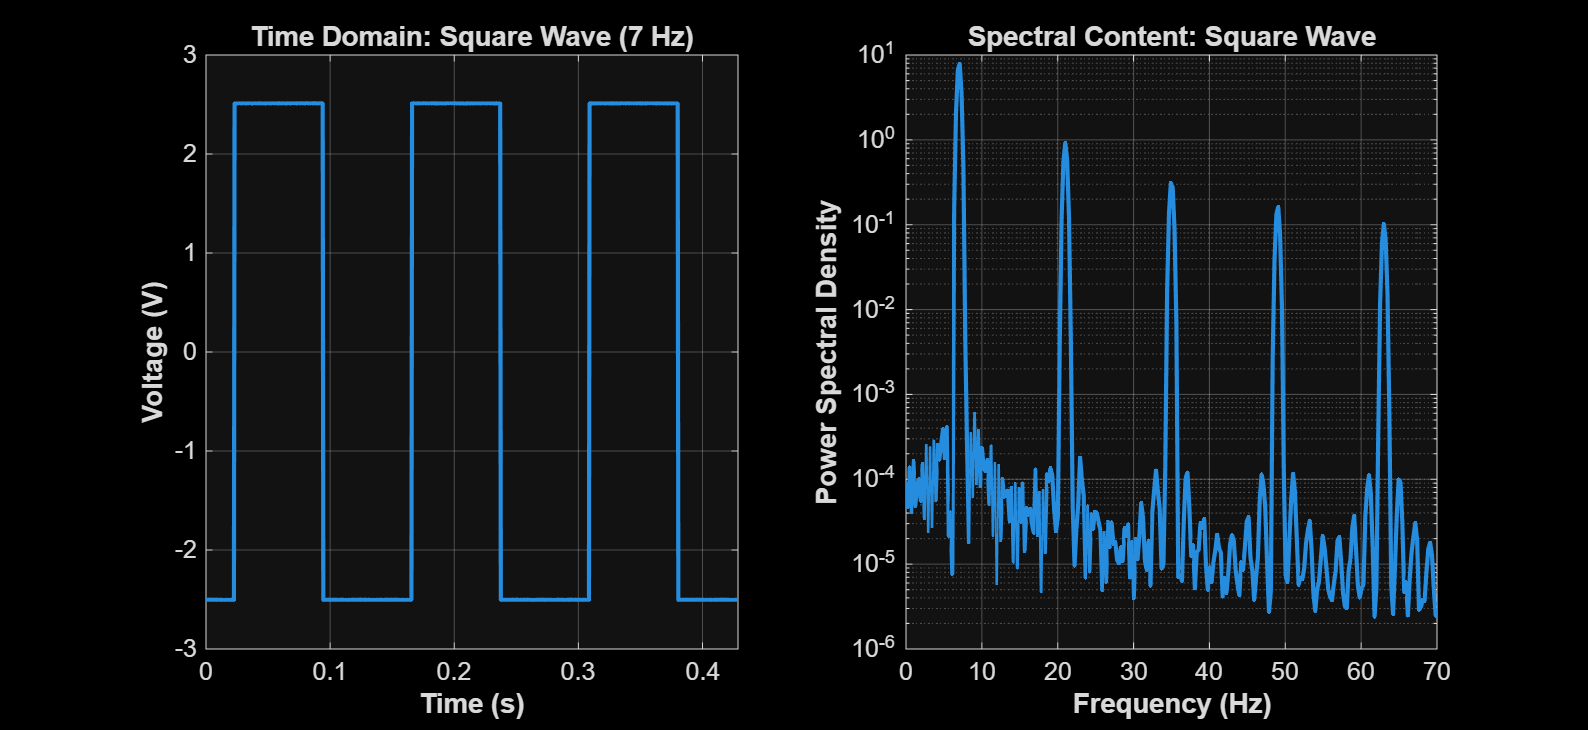
\includegraphics[width=0.9\textwidth]{../pictures/Square_7Hz_5.0Vpp_0.0Voffset.png}
  \caption{Square Wave (\SI{7}{\hertz}) Analysis.}
\end{figure}

\begin{table}[H]
  \centering
  \begin{tabular}{ccc}
    \toprule
    \textbf{Mean Voltage} & \textbf{RMS Voltage} & \textbf{DC Offset} \\
    \midrule
    \SI{0.0045}{\volt} & \SI{2.5065}{\volt} & \SI{0.0045}{\volt} \\
    \bottomrule
  \end{tabular}
\end{table}

% ---------------------------------------------------------
% Signal 8: Square 25Hz
% ---------------------------------------------------------
\subsection*{8. Square Wave: \SI{25}{\hertz}, \SI{0.3}{V_{pp}}, \SI{0.2}{V} Offset}

\begin{figure}[H]
  \centering
  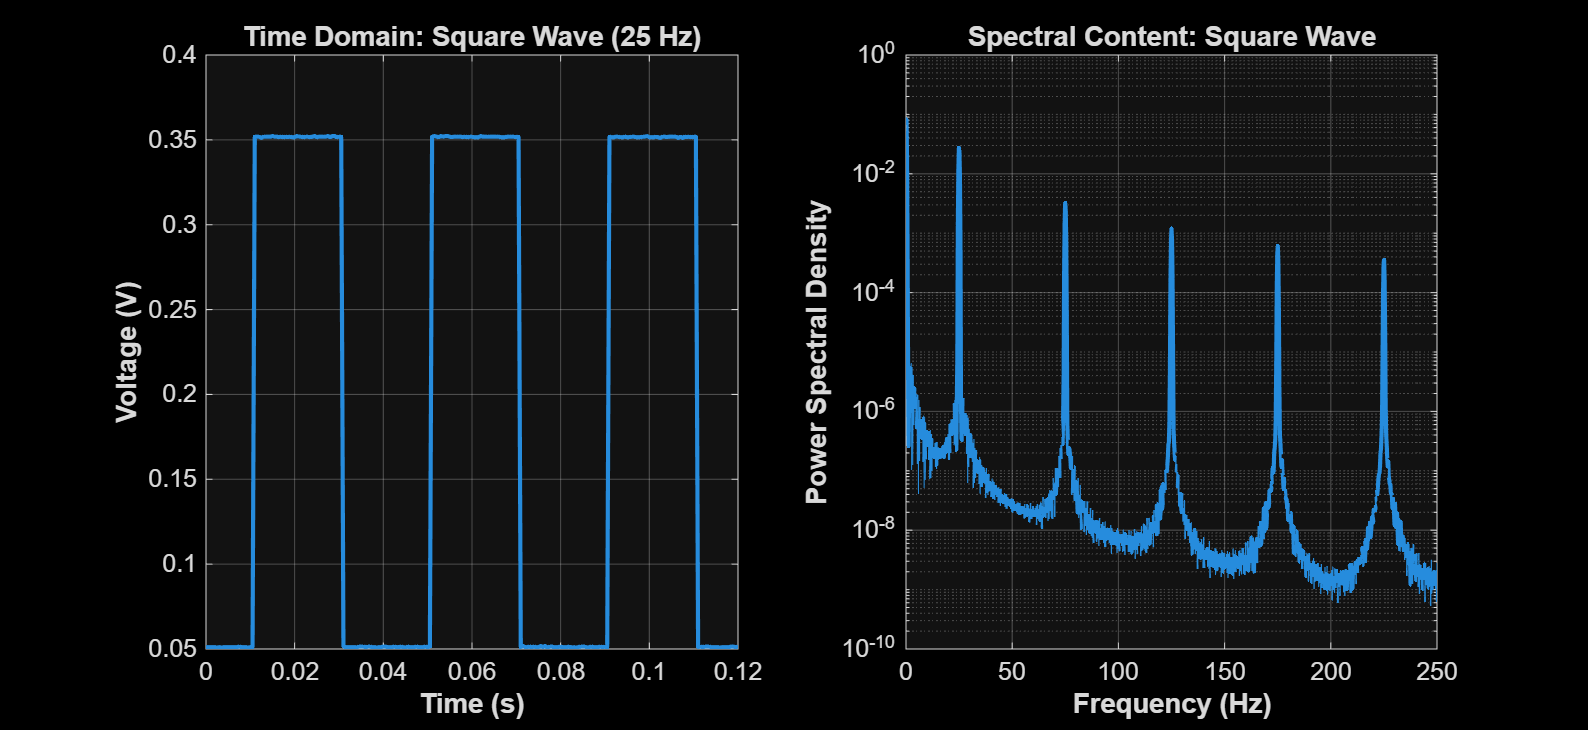
\includegraphics[width=0.9\textwidth]{../pictures/Square_25Hz_0.3Vpp_0.2Voffset.png}
  \caption{Square Wave (\SI{25}{\hertz}) Analysis.}
\end{figure}

\begin{table}[H]
  \centering
  \begin{tabular}{ccc}
    \toprule
    \textbf{Mean Voltage} & \textbf{RMS Voltage} & \textbf{DC Offset} \\
    \midrule
    \SI{0.2014}{\volt} & \SI{0.2513}{\volt} & \SI{0.2014}{\volt} \\
    \bottomrule
  \end{tabular}
\end{table}

\newpage
\section*{Part 2: Discussion and Spectral Analysis}

\textbf{1. Choice of Y-Axis Scale (Linear vs. Logarithmic)}\\
A logarithmic (dB) scale was explicitly chosen for the y-axis of all power spectrum plots . This is an engineering necessity when performing Fourier analysis on non-sinusoidal waveforms. While a linear scale clearly displays the fundamental frequency, the higher-order harmonics (which mathematically dictate the physical shape of the wave) often contain orders of magnitude less energy. On a linear scale, these critical harmonics visually collapse into the noise floor. A logarithmic scale compresses this massive dynamic range, allowing the distinct structural decay rates of the harmonics to be clearly identified and analyzed.

\textbf{2. Square Wave vs. Ramp Wave (Identical Frequency/Amplitude)}\\
While a square wave and a ramp wave share the same fundamental frequency peak, their harmonic content differs drastically. A square wave consists exclusively of \textit{odd} harmonics ($3f, 5f, 7f\dots$), and its amplitude rolls off at a rate proportional to $1/n$ (power $\propto 1/n^2$). Conversely, depending on its symmetry, a ramp wave contains a different spectral density. The sharp, instantaneous transitions of the square wave require more high-frequency energy to recreate mathematically, meaning the harmonic peaks in the square wave's spectrum decay slower and are more prominent at higher frequencies compared to a 50\% triangle wave.

\textbf{3. Effect of Ramp Wave Symmetry (50\% vs. 100\%)}\\
Altering the symmetry of the ramp wave fundamentally changes its spectral signature .
\begin{itemize}
  \item \textbf{50\% Symmetry (Triangle Wave):} Because the wave is perfectly symmetric, it contains \textit{only odd harmonics}. Furthermore, its harmonic amplitude rolls off rapidly, proportional to $1/n^2$ (meaning power rolls off as $1/n^4$). The spectrum appears sparse and decays very quickly.
  \item \textbf{100\% Symmetry (Sawtooth Wave):} This wave features a slow linear rise followed by an instantaneous vertical drop. This sharp discontinuity requires \textit{both even and odd harmonics} to reconstruct. Its amplitude rolls off much slower, proportional to $1/n$. Thus, the 100\% ramp spectrum is heavily saturated with dense, prominent peaks across the entire frequency band.
\end{itemize}

\textbf{4. Square Waves at Different Frequencies and Amplitudes}\\
When comparing the \SI{7}{\hertz} (\SI{5.0}{V_{pp}}) square wave to the \SI{25}{\hertz} (\SI{0.3}{V_{pp}}) square wave, the underlying mathematical architecture remains identical. Both spectrums exhibit energy exclusively at odd integer multiples of their respective fundamental frequencies. Changing the frequency merely shifts the physical location of the fundamental peak (from \SI{7}{\hertz} to \SI{25}{\hertz}) and expands the absolute distance between subsequent harmonics. Changing the amplitude universally scales the magnitude of all peaks on the y-axis, but the \textit{relative ratio} of power between the fundamental frequency and its harmonics remains perfectly constant.

\textbf{5. The Effect of DC Offset on the Spectral Plot}\\
A DC offset is mathematically equivalent to a signal with a frequency of \SI{0}{\hertz}. When analyzing the \SI{7}{\hertz} signals (which had \SI{0.0}{\volt} offset), the power spectrum drops off cleanly near the y-axis. However, the \SI{25}{\hertz} signals were injected with a \SI{0.2}{\volt} DC offset. This manifests in the spectral plot as a massive, distinct power spike at exactly \SI{0}{\hertz}. The amplitude of this \SI{0}{\hertz} bin in the Fourier transform directly corresponds to the calculated Mean Voltage (\SI{\approx 0.2}{\volt}) reported in the data tables.

\newpage
\appendix
\section*{Appendix: MATLAB Signal Analysis Code}
The following MATLAB scripts were utilized to acquire the raw DAQ data, iteratively compute the statistical parameters across all matrices, and generate the paired time-domain and logarithmic frequency-domain plots.

\subsection*{lab4\_RecordData.m}
\lstinputlisting[language=Matlab]{../lab4_RecordData.m}

\subsection*{lab4\_Analysis.m}
\lstinputlisting[language=Matlab]{../lab4_Analysis.m}

\end{document}
